% !TEX TS-program = knitr
\documentclass[handout]{beamer}\usepackage[]{graphicx}\usepackage[]{color}
% maxwidth is the original width if it is less than linewidth
% otherwise use linewidth (to make sure the graphics do not exceed the margin)
\makeatletter
\def\maxwidth{ %
  \ifdim\Gin@nat@width>\linewidth
    \linewidth
  \else
    \Gin@nat@width
  \fi
}
\makeatother

\definecolor{fgcolor}{rgb}{0.345, 0.345, 0.345}
\newcommand{\hlnum}[1]{\textcolor[rgb]{0.686,0.059,0.569}{#1}}%
\newcommand{\hlstr}[1]{\textcolor[rgb]{0.192,0.494,0.8}{#1}}%
\newcommand{\hlcom}[1]{\textcolor[rgb]{0.678,0.584,0.686}{\textit{#1}}}%
\newcommand{\hlopt}[1]{\textcolor[rgb]{0,0,0}{#1}}%
\newcommand{\hlstd}[1]{\textcolor[rgb]{0.345,0.345,0.345}{#1}}%
\newcommand{\hlkwa}[1]{\textcolor[rgb]{0.161,0.373,0.58}{\textbf{#1}}}%
\newcommand{\hlkwb}[1]{\textcolor[rgb]{0.69,0.353,0.396}{#1}}%
\newcommand{\hlkwc}[1]{\textcolor[rgb]{0.333,0.667,0.333}{#1}}%
\newcommand{\hlkwd}[1]{\textcolor[rgb]{0.737,0.353,0.396}{\textbf{#1}}}%
\let\hlipl\hlkwb

\usepackage{framed}
\makeatletter
\newenvironment{kframe}{%
 \def\at@end@of@kframe{}%
 \ifinner\ifhmode%
  \def\at@end@of@kframe{\end{minipage}}%
  \begin{minipage}{\columnwidth}%
 \fi\fi%
 \def\FrameCommand##1{\hskip\@totalleftmargin \hskip-\fboxsep
 \colorbox{shadecolor}{##1}\hskip-\fboxsep
     % There is no \\@totalrightmargin, so:
     \hskip-\linewidth \hskip-\@totalleftmargin \hskip\columnwidth}%
 \MakeFramed {\advance\hsize-\width
   \@totalleftmargin\z@ \linewidth\hsize
   \@setminipage}}%
 {\par\unskip\endMakeFramed%
 \at@end@of@kframe}
\makeatother

\definecolor{shadecolor}{rgb}{.97, .97, .97}
\definecolor{messagecolor}{rgb}{0, 0, 0}
\definecolor{warningcolor}{rgb}{1, 0, 1}
\definecolor{errorcolor}{rgb}{1, 0, 0}
\newenvironment{knitrout}{}{} % an empty environment to be redefined in TeX

\usepackage{alltt}
\setbeamercovered{dynamic}
\newcommand{\answers}{1}

\usetheme{Marburg}
\setbeamertemplate{navigation symbols}{} 
\setbeamertemplate{footline}
{
  \leavevmode%
  \hbox{%
  \begin{beamercolorbox}[wd=.333333\paperwidth,ht=2.25ex,dp=1ex,center]{author in head/foot}%
    \usebeamerfont{author in head/foot} $\ $ \insertshortauthor%~~\beamer@ifempty{\insertshortinstitute}{}{(\insertshortinstitute)}
  \end{beamercolorbox}%
  \begin{beamercolorbox}[wd=.333333\paperwidth,ht=2.25ex,dp=1ex,center]{title in head/foot}%
    \usebeamerfont{title in head/foot} \insertinstitute
  \end{beamercolorbox}%
  \begin{beamercolorbox}[wd=.333333\paperwidth,ht=2.25ex,dp=1ex,right]{date in head/foot}%
    \usebeamerfont{date in head/foot}\insertshortdate{}\hspace*{2em}
    \insertframenumber{} / \inserttotalframenumber\hspace*{2ex} 
  \end{beamercolorbox}}%
  \vskip0pt%
}

\usepackage{amsmath}
\usepackage{caption}
\usepackage{color}
\usepackage{enumerate}
\usepackage{listings}
\usepackage{hyperref}
\usepackage{mathrsfs}
\usepackage{natbib}
\usepackage{url}

\providecommand{\all}{\ \forall \ }
\providecommand{\bs}{\backslash}
\providecommand{\e}{\varepsilon}
\providecommand{\E}{\ \exists \ }
\providecommand{\lm}[2]{\lim_{#1 \rightarrow #2}}
\providecommand{\m}[1]{\mathbb{#1}}
\providecommand{\nv}{{}^{-1}}
\providecommand{\ov}[1]{\overline{#1}}
\providecommand{\p}{\newpage}
\providecommand{\q}{$\quad$ \newline}
\providecommand{\rt}{\rightarrow}
\providecommand{\Rt}{\Rightarrow}
\providecommand{\vc}[1]{\boldsymbol{#1}}
\providecommand{\wh}[1]{\widehat{#1}}

\hypersetup{colorlinks,linkcolor=,urlcolor=blue}
\numberwithin{equation}{section}

\definecolor{dkgreen}{rgb}{0,0.6,0}
\definecolor{gray}{rgb}{0.5,0.5,0.5}
\definecolor{mauve}{rgb}{0.58,0,0.82}

\lstset{ 
  language=C,                % the language of the code
  basicstyle= \footnotesize,           % the size of the fonts that are used for the code
  numberstyle= \tiny \color{white},  % the style that is used for the line-numbers
  stepnumber=2,                   % the step between two line-numbers. 
  numbersep=5pt,                  % how far the line-numbers are from the code
  backgroundcolor=\color{white},      % choose the background color. You must add \usepackage{color}
  showspaces=false,               % show spaces adding particular underscores
  showstringspaces=false,         % underline spaces within strings
  showtabs=false,                 % show tabs within strings adding particular underscores
  frame=lrb,                   % adds a frame around the code
  rulecolor=\color{black},        % if not set, the frame-color may be changed on line-breaks within not-black text 
  tabsize=2,                      % sets default tabsize to 2 spaces
  captionpos=t,                   % sets the caption-position 
  breaklines=true,                % sets automatic line breaking
  breakatwhitespace=false,        % sets if automatic breaks should only happen at whitespace
  %title=\lstname,                   % show the filename of files included with \lstinputlisting;
  keywordstyle=\color{blue},          % keyword style
  commentstyle=\color{gray},       % comment style
  stringstyle=\color{dkgreen},         % string literal style
  escapeinside={\%*}{*)},            % if you want to add LaTeX within your code
  morekeywords={*, ...},               % if you want to add more keywords to the set
  xleftmargin=0.053in, % left horizontal offset of caption box
  xrightmargin=-.03in % right horizontal offset of caption box
}

%\DeclareCaptionFont{white}{\color{white}}
%\DeclareCaptionFormat{listing}{\parbox{\textwidth}{\colorbox{gray}{\parbox{\textwidth}{#1#2#3}}\vskip-0.05in}}
%\captionsetup[lstlisting]{format = listing, labelfont = white, textfont = white}
%For caption-free listings, comment out the 3 lines above and uncomment the 2 lines below.
 \captionsetup{labelformat = empty, labelsep = none}
 \lstset{frame = single}





\title{Functions of Several Random Variables (Ch. 5.5)}
\author{Yifan Zhu}
\date{}
\institute{Iowa State University}
\IfFileExists{upquote.sty}{\usepackage{upquote}}{}
\begin{document}

\begin{frame}
\titlepage
 \end{frame}
 
 \AtBeginSection[]
{
   \begin{frame}
       \frametitle{Outline}
       \tableofcontents[currentsection]
   \end{frame}
}

\section{Functions of Several Random Variables}

\begin{frame}
\frametitle{Functions of several random variables}
\begin{itemize}
\pause \item We often consider functions of random variables of the form:
\pause \begin{align*}
U = g(X, Y, \ldots, Z)
\end{align*}
\pause where $X$, $Y, \ldots, Z$ are random variables.
\pause \item $U$ is itself a random variable.
\end{itemize}
\end{frame}


\begin{frame}
\frametitle{Example: connecting steel parts}
\begin{itemize}
\item Suppose that a steel plate with nominal thickness .15 in. is to rest in a groove of nominal width .155 in., machined on the surface of a steel block. \q \q
\setkeys{Gin}{width=.45\textwidth} 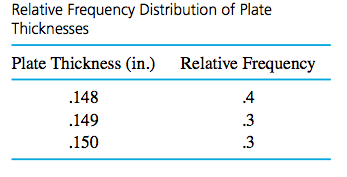
\includegraphics{../../fig/platet.png}
\setkeys{Gin}{width=.45\textwidth} 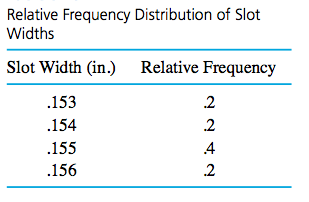
\includegraphics{../../fig/slott.png}
\pause \item $X$ = plate thickness
\pause \item $Y$ = slot width
\pause \item $U=Y-X$, the ``wiggle room" of the plate
\end{itemize}
\end{frame}

\begin{frame}
\frametitle{The distributions of $X$, $Y$, and $U$}
\setkeys{Gin}{width=.45\textwidth} 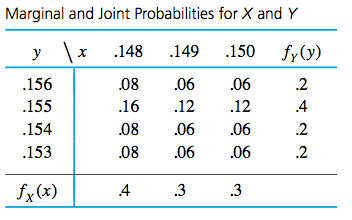
\includegraphics{../../fig/platexy.png}
\setkeys{Gin}{width=.45\textwidth} 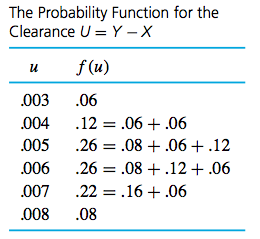
\includegraphics{../../fig/plateu.png}
\begin{itemize}
\pause \item Determining the distribution of $U$ is difficult in the continuous case.
\end{itemize}
\end{frame}




\section{Expectations and variances of linear combinations}


\begin{frame}
\frametitle{Expectations and variances of linear combinations}
\begin{itemize}
\pause \item $X_1, X_2, \ldots, X_n$ are independent random variables and
\pause \begin{align*}
Y = a_0 + a_1 X_1 + a_2 X_2 + \cdots + a_n X_n
\end{align*} 
\pause then:
\begin{align*}
\uncover<4->{E(Y)} & \uncover<4->{= E(a_0 + a_1 X_1 + a_2 X_2 + \cdots + a_n X_n)} \\
&\uncover<5->{= a_0 + a_1 E(X_1) + a_2 E(X_2) + \cdots + a_n E(X_n)} \\ \\
\uncover<6->{Var(Y)} & \uncover<6->{= Var(a_0 + a_1 X_1 + a_2 X_2 + \cdots + a_n X_n)} \\
&\uncover<7->{= a_1^2 \cdot Var(X_1) + a_2^2  \cdot Var(X_2) + \cdots + a_n^2 \cdot Var(X_n)}
\end{align*}
\end{itemize}
\end{frame}



\begin{frame}
\frametitle{Your turn: linear combinations}
\begin{itemize}
\item Say we have two independent random variables $X$ and $Y$ with $E(X) = 3.3, Var(X) = 1.91, E(Y) = 25$, and $Var(Y) = 65$.
\item Find:
\begin{align*}
E(3 + 2X - 3Y) \\
E(-4 X + 3Y) \\
E(-4X - 6Y) \\
Var(3 + 2X - 3Y) \\ 
Var(2X - 5Y) \\
Var(-4X - 6Y)  
\end{align*}
\end{itemize}
\end{frame}

\begin{frame}<handout:\answers>
\frametitle{Answers: linear combinations}
\begin{align*}
E(3 + 2X - 3Y) &= 3 + 2 E(X) - 3 E(Y) \\
& \uncover<2->{= 3 + 2 \cdot 3.3 - 3 \cdot 25} \\
& \uncover<3->{= -65.4} \\ \\
\uncover<4->{E(-4 X + 3Y)} & \uncover<4->{= -4 E(X) + 3 E(Y)} \\
&\uncover<5->{ = -4 \cdot 3.3 + 3 \cdot 25} \\
&\uncover<6->{ = 61.8} \\ \\
\uncover<7->{E(-4X - 6Y)} & \uncover<7->{ = -4 \cdot E(X) - 6 \cdot E(Y)} \\
& \uncover<8->{= -4 \cdot 3.3 - 6 \cdot 25} \\
& \uncover<9->{= -163.2}
\end{align*}
\end{frame}

\begin{frame}<handout:\answers>
\frametitle{Answers: linear combinations}
\begin{align*}
Var(3 + 2X - 3Y) &= 2^2 \cdot Var(X) + (-3)^2 Var(Y) \\ 
&\uncover<2->{ = 4 \cdot 1.91 + 9 \cdot 65} \\
& \uncover<3->{= 592.64} \\ \\
\uncover<4->{Var(2X - 5Y)} & \uncover<4->{= 2^2 \cdot Var(X) + (-5)^2 Var(Y)} \\
& \uncover<5->{= 4 \cdot 1.91 + 25 \cdot 65} \\
& \uncover<6->{= 1632.64} \\ \\
\uncover<7->{Var(-4X - 6Y)} & \uncover<7->{= (-4)^2 \cdot Var(X) + (-6)^2 Var(Y)} \\
& \uncover<8->{= 16 \cdot 1.91 + 36 \cdot 65} \\
&\uncover<9->{ = 2370.56}
\end{align*} 
\end{frame}


\begin{frame}
\frametitle{Your turn: more linear combinations}
\begin{itemize}
\item Say $X \sim$ Binomial($n= 10$, $p = 0.5$) and $Y \sim$ Poisson($\lambda = 3$).
\item Calculate:
\end{itemize}
\begin{align*}
E(5 + 2X - 7 Y) \\
Var(5 + 2X - 7 Y)
\end{align*}
\end{frame}

\begin{frame}<handout:\answers>
\frametitle{Answer: more linear combinations}
\begin{itemize}
\item First, note that:
\end{itemize}
\begin{align*}
\uncover<2->{E(X)} & \uncover<2->{= np} \uncover<3->{ = 10 \cdot 0.5 = 5} \\
\uncover<3->{E(Y)} & \uncover<3->{= \lambda = 3} \\
\uncover<4->{Var(X)} & \uncover<4->{= np(1-p)} \uncover<4->{ = 10(0.5)(1-0.5) = 2.5} \\
\uncover<5->{Var(Y)} &\uncover<5->{= \lambda = 3}
\intertext{\uncover<6->{Now, we can calculate:}}
\uncover<7->{E(5 + 2X - 7 Y)} &  \uncover<7->{= 5 + 2 E(X) - 7 E(Y)} \\
& \uncover<8->{= 5 + 2 \cdot 5 - 7 \cdot 3} \\
&\uncover<9->{ = -6} \\ \\
\uncover<10->{Var(5 + 2X - 7 Y)} & \uncover<10->{= 2^2 \cdot Var(X) + (-7)^2 \cdot Var(Y)} \\ 
&\uncover<11->{= 4 \cdot 2.5 + 49 \cdot 3} \\ 
&\uncover<12->{ = 157}
\end{align*}
\end{frame}

\section{Approximating the Mean and Variance of a Function}

\begin{frame}
\frametitle{\small Approximating $E(U)$ and $Var(U)$ when determining $f_U(u)$ is too hard} \scriptsize
\begin{itemize}
\pause \item If $X, Y, \ldots, Z$ are independent, $g$ is well-behaved, and the variances Var$(X)$, Var$(Y), \ldots,$ Var($Z$) are small enough, then $U = g(X, Y, \ldots Z)$ has:
\begin{align*}
\uncover<3->{E(U)} &\uncover<3->{\approx g(E(X), E(Y), \ldots, E(Z))} \\
\uncover<4->{\text{Var}(U)} & \uncover<4->{\approx \left ( \frac{\partial g}{\partial x}\right )^2 Var(X) + \left ( \frac{\partial g}{\partial y}\right )^2 Var(Y) + \cdots + \left ( \frac{\partial g}{\partial z}\right )^2 Var(Z)}
\end{align*}
\uncover<5->{\item These formulas are often called the {\bf propagation of error formulas}.}
\end{itemize}
\end{frame}

\begin{frame}
\frametitle{Example: an electric circuit}
\begin{center}
\setkeys{Gin}{width=.6\textwidth} 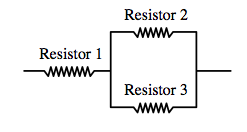
\includegraphics{../../fig/resist.png}
\end{center}
\begin{itemize}
\pause \item $R$ is the total resistance of the circuit.
\pause \item $R_1$, $R_2$, and $R_3$ are the resistances of resistors 1, 2, and 3, respectively.
\pause \item $E(R_i) = 100$, Var($R_i)$ = 2, $i = 1,2,3$. 
\end{itemize}
\pause \begin{align*}
R = g(R_1, R_2, R_3) = R_1 + \frac{R_2 R_3}{R_2 + R_3}
\end{align*}
\end{frame}

\begin{frame}
\frametitle{Example: an electric circuit} \scriptsize
\begin{align*}
E(R) &\approx g(100, 100, 100) \uncover<2->{= 100 + \frac{(100)(100)}{100 + 100}} \uncover<3->{= 150 \Omega} \\
\uncover<4->{\frac{\partial g}{\partial r_1}} & \uncover<4->{= 1} \\
\uncover<5->{\frac{\partial g}{\partial r_2}} & \uncover<5->{= \frac{(r_2 + r_3)r_3 - r_2r_3}{(r_2 + r_3)^2}}\uncover<6->{ = \frac{r_3^2}{(r_2 + r_3)^2}} \\
\uncover<7->{\frac{\partial g}{\partial r_3}} & \uncover<7->{= \frac{(r_2 + r_3)r_2 - r_2 r_3}{(r_2 + r_3)^2}} \uncover<8->{ = \frac{r_2^2}{(r_2 + r_3)^2}} \\
\uncover<9->{\text{Var(R)}} &\uncover<9->{ \approx (1)^2 (2)^2 + \left ( \frac{(100)^2}{(100 + 100)^2} \right ) ^2 (2)^2 + \left (\frac{(100)^2}{(100 + 100)^2} \right ) ^2 (2)^2 } \\
&\uncover<10->{= 4.5} \\
\uncover<11->{\text{SD}(R)} &\uncover<11->{\sqrt{4.5} \approx 2.12 \Omega}
\end{align*}
\end{frame}











\section{The Central Limit Theorem}

\begin{frame}
\frametitle{iid random variables.}
\begin{itemize}
\pause \item {\bf Identically Distributed}: Random variables $X_1, X_2, \ldots, X_n$ are identically distributed if they have the same probability distribution.
\pause \item {\bf ``iid"}: Random variables $X_1, X_2, \ldots, X_n$ are iid if they are {\bf I}ndependent and {\bf I}dentically {\bf D}istributed. 
\end{itemize}
\end{frame}



\begin{frame}
\frametitle{Averages of iid random variables}

\begin{itemize}
\item $X_1, X_2, \ldots, X_n$ are iid with expectation $\mu$ and variance $\sigma^2$.
\item Derive:
\end{itemize}

\begin{align*}
&E(\ov{X}) \\
&Var(\ov{X}) 
\intertext{where:}
\ov{X} &= \frac{X_1 + X_2 + \cdots + X_n}{n}
\intertext{the mean of the $X_i$'s.}
\end{align*}
\end{frame}

\begin{frame}<handout:\answers>
\frametitle{Averages of iid random variables}\scriptsize
\begin{align*}
E(\ov{X}) &= E \left (\frac{X_1 + X_2 + \cdots + X_n}{n} \right) \\ 
&\uncover<2->{ = \frac{1}{n} E(X_1) + \frac{1}{n}E(X_2) + \cdots + \frac{1}{n}E(X_n)} \\ 
&\uncover<3->{ = \underbrace{\frac{1}{n} \mu +  \frac{1}{n} \mu + \cdots + \frac{1}{n} \mu}_{n\text{ times}}} \\ 
&\uncover<4->{ = n \cdot \frac{1}{n} \mu} \\ 
&\uncover<5->{ = \fbox{\color{blue}$\mu$}}
\end{align*}
\begin{itemize}
\uncover<6->{\item Remember $E(\ov{X}) = \mu$: it's an important result.}
\end{itemize}
\end{frame}

\begin{frame}<handout:\answers>
\frametitle{Answers: averages of iid random variables} \scriptsize
\begin{align*}
Var(\ov{X}) &= Var \left (\frac{X_1 + X_2 + \cdots + X_n}{n} \right) \\ 
&\uncover<2->{ = \left (\frac{1}{n}\right )^2 Var(X_1) + \left (\frac{1}{n}\right )^2 Var(X_2) + \cdots + \left (\frac{1}{n}\right )^2  \cdot Var(X_n)} \\ 
& \uncover<3->{= \underbrace{\frac{1}{n^2} \sigma^2 +  \frac{1}{n^2} \sigma^2 + \cdots + \frac{1}{n^2} \sigma^2}_{n\text{ times}}} \\ 
& \uncover<4->{= n \cdot \frac{1}{n^2} \sigma^2} \\ 
& \uncover<5->{= \fbox{ \color{blue} $\frac{\sigma^2}{n}$}}
\end{align*}
\begin{itemize}
\uncover<6->{\item Remember $Var(\ov{X}) = \frac{\sigma^2}{n}$: it's another important result.}
\end{itemize}
\end{frame}


\begin{frame}
\frametitle{Example: length of seeds}
\begin{itemize}
\item A botanist has collected a sample of 10 seeds and measures the length of each. 
\pause \item The seed lengths  $X_1, X_2, \ldots, X_{10}$ are supposed to be iid with mean $\mu = 5$ mm and variance $\sigma^2 = 2$ $mm^2$.
\begin{align*}
&\uncover<3->{E(\ov{X}) = \mu = 5 }\\
& \uncover<4->{Var(\ov{X}) =\sigma^2/n} \uncover<5->{= 2/10 = 0.2}
\end{align*} $\quad$ \newline
\end{itemize}
\end{frame}


\begin{frame}
\frametitle{The Central Limit Theorem}
\begin{itemize}
\pause \item If $X_1, X_2, \ldots, X_n$ are \emph{any} iid random variables with mean $\mu$ and variance $\sigma^2 < \infty$, and if $n \ge 25$, 
\pause \begin{align*}
\ov{X} \approx \text{Normal} \left (\mu, \frac{\sigma^2}{n} \right)
\end{align*}
\pause \item The Central Limit Theorem (CLT) one of the most important and useful results in statistics.
\end{itemize}
\end{frame}


\begin{frame}
\frametitle{Example: tool serial numbers}
\begin{itemize}
\pause \item $W_1$ = last digit of the serial number observed next Monday at 9 AM
\pause \item $W_2$ = last digit of the serial number the Monday after at 9 AM
\pause \item $W_1 $ and $ W_2$ are independent with pmf:
\pause \begin{align*}
f(w) = \begin{cases}
0.1 & w = 0, 1, 2, \ldots, 9 \\
0 & \text{otherwise} 
\end{cases}
\end{align*}
\pause \item $\ov{W} = \frac{1}{2}(W_1 + W_2)$ has the pmf:
\end{itemize}
\setkeys{Gin}{width=.95\textwidth} 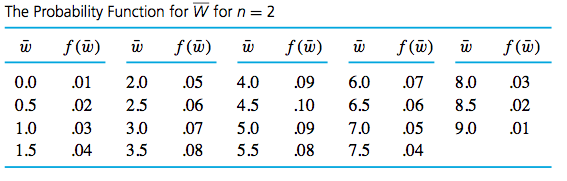
\includegraphics{../../fig/wpmf.png}
\end{frame}

\begin{frame}
\frametitle{Example: tool serial numbers}
\setkeys{Gin}{width=.45\textwidth} 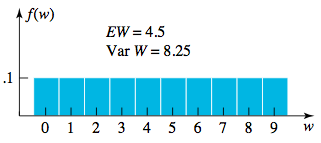
\includegraphics{../../fig/wbar1.png}
\setkeys{Gin}{width=.45\textwidth} 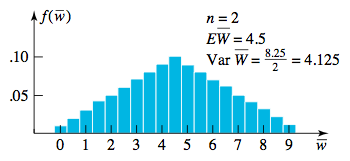
\includegraphics{../../fig/wbar2.png}
\begin{itemize}
\item What if $\ov{W} = \frac{1}{8}(W_1 + W_2 + \cdots + W_8)$, the average of 8 days of initial serial numbers?
\end{itemize}
\setkeys{Gin}{width=.7\textwidth} 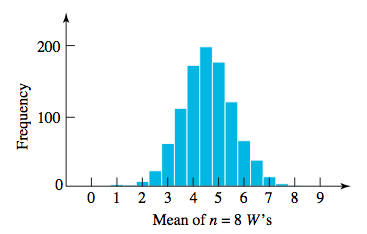
\includegraphics{../../fig/wbar8.png}
\end{frame}


\begin{frame}
\frametitle{Example: excess sale time}
\begin{itemize}
\pause \item $\ov{S}$ = sample mean excess sale time (over a 7.5 s threshold) for 100 stamp sales.
\pause \item Each individual excess sale time should have an Exp($\alpha = 16.5$ s) distribution. That means:
\begin{itemize}
\pause \item $E(\ov{S}) = \alpha = 16.5$ s
\pause \item $SD(\ov{S}) = \sqrt{\text{Var}(\ov{S})} = \sqrt{\frac{\alpha^2}{100}} = 1.65$ s
\pause \item By the Central Limit Theorem, $\ov{S} \approx N(16.5, 1.65^2)$
\end{itemize}
\pause \item We want to approximate $P(\ov{S} > 17)$.
\end{itemize}
\setkeys{Gin}{width=.8\textwidth} 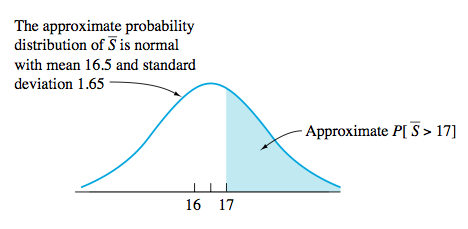
\includegraphics{../../fig/salesnorm.png}
\end{frame}


\begin{frame}
\frametitle{Example: excess sale time}
\begin{align*}
P(\ov{S} > 17) &= P(\frac{\ov{S} - 16.5}{1.65} > \frac{17 - 16.5}{1.65})\\
&\uncover<2->{\approx P(Z > 0.303) \qquad (Z \sim N(0,1))} \\
&\uncover<3->{= 1 - P(Z \le 0.303)} \\
& \uncover<4->{= 1 - \Phi(0.303)} \\
&\uncover<5->{ = 1 - 0.62 \quad \text{from the standard normal table} }\\
&\uncover<6->{= 0.38}
\end{align*}
\end{frame}

\begin{frame}
\frametitle{Example: net weight of baby food jars}
\begin{itemize}
\item Individual jar weights are iid with unknown mean $\mu$ and standard deviation $\sigma = 1.6$ g 
\pause \item $\ov{V}$ = sample mean weight of n jars $\approx N \left (\mu, \frac{1.6^2}{n} \right )$.
\pause \item We want to find $\mu$. One way to hone in on $\mu$ is to find $n$ such that:
\pause \begin{align*}
P(\mu - 0.3 < \ov{V} < \mu + 0.3) = 0.8
\end{align*}
\pause That way, our measured value of $\ov{V}$ is likely to be close to $\mu$. 
\end{itemize}
\end{frame}

\begin{frame}
\frametitle{Example: net weight of baby food jars} \small
\begin{align*}
0.8 &= P(\mu - 0.3 < \ov{V} < \mu + 0.3) \\
&\uncover<2->{= P(\frac{-0.3}{1.6/\sqrt{n}} < \frac{\ov{V} - \mu}{1.6/\sqrt{n}} < \frac{0.3}{1.6/\sqrt{n}} )} \\
&\uncover<3->{\approx P(-0.19 \sqrt{n} < Z < 0.19 \sqrt{n} ) \quad \text{(by CLT)} }\\
&\uncover<4->{= 1 - 2\Phi(-0.19 \sqrt{n}) \quad \text{(look at the N(0,1) pdf)}} \\
\uncover<5->{\Phi \nv (0.1)} & \uncover<5->{= -0.19 \sqrt{n} }\\
\uncover<6->{n} & \uncover<6->{= \frac{\Phi \nv (0.1)^2}{(-0.19)^2}} \\
&\uncover<7->{= \frac{(-1.28)^2}{(-0.19)^2} \quad \text{(standard normal table)}} \\
&\uncover<8->{= 46.10}
\end{align*}
\begin{itemize}
\uncover<9->{ \item Hence, we'll need a sample size of $n= 47$.}
\end{itemize}
\end{frame}


\begin{frame}
\frametitle{Example: cars}
\begin{itemize}
\pause \item Suppose a bunch of cars pass through certain stretch of road. Whenever a car comes, you look at your watch and record the time. 
\pause \item Let $X_i$ be the time (in hours) between when the $i$'th car comes and the $(i + 1)$'th car comes, $i = 1, \ldots, 44$. Suppose you know:

\pause \pause \begin{align*}
X_1, X_2, \ldots, X_{44} \sim \text{ iid } f(x) = e^{-x} \quad x \ge 0 \\
\end{align*} $\quad$

\pause \item Find the probability that the average time gap between cars exceeds 1.05 hours.
\end{itemize}
\end{frame}


\begin{frame}
\frametitle{Example: cars}
\begin{align*}
\mu &= E(X_1) \\ \\
&\uncover<2->{= \int_{-\infty}^\infty x f(x) dx} \\ \\
&\uncover<3->{= \int_{0}^\infty x e^{-x} dx} \\ \\
&\uncover<4->{= -e^{-x}(x+1)|_{0}^{\infty} \quad \text{ integration by parts }} \\ \\
&\uncover<5->{ = 1}
\end{align*}
\end{frame}


\begin{frame}
\frametitle{Example: cars}
\begin{align*}
E(X_1^2) &= \int_{-\infty}^\infty x^2 f(x) dx \\ 
&\uncover<2->{= \int_{0}^\infty x^2 e^{-x} dx} \\ 
&\uncover<3->{= -e^{-x}(x^2 + 2x + 2)|_{0}^{\infty} \quad \text{ integration by parts }} \\ 
&\uncover<4->{ = 2} \\
\uncover<5->{\sigma^2} & \uncover<5->{= Var(X_1)} \\
&\uncover<6->{= E(X_1^2) - E^2(X_1)} \\
& \uncover<7->{= 2 - 1^2} \\
& \uncover<8->{= 1}
\end{align*}
\end{frame}



\begin{frame}
\frametitle{Example: cars}
\begin{align*}
\ov{X} &\sim \text{ approx. } N(\mu, \sigma^2/n) \\
&\uncover<2->{ = N(1, 1/44)}
\intertext{\uncover<3->{Thus:}}
\uncover<3->{\frac{\ov{X}-1}{\sqrt{1/44}}} & \uncover<4->{\sim N(0,1)}
\end{align*}
\end{frame}

\begin{frame}
\frametitle{Example: cars}
\begin{align*}
\intertext{Now, we're ready to approximate:}
P(\ov{X} > 1.05) & = P(\frac{\ov{X}-1}{\sqrt{1/44}} > \frac{1.05-1}{\sqrt{1/44}}) \\ 
&\uncover<2->{ = P(\frac{\ov{X}-1}{\sqrt{1/44}} > 0.332)} \\
&\uncover<3->{ \approx P(Z > 0.332)} \\ 
& \uncover<4->{= 1- P(Z \le 0.332)} \\ 
& \uncover<5->{= 1- \Phi(0.332)} \\ 
&\uncover<6->{ = 1- 0.630 = 0.370}
\end{align*}
\end{frame}

\begin{frame}[fragile]
\frametitle{Example: cars}
\begin{knitrout}
\definecolor{shadecolor}{rgb}{0.969, 0.969, 0.969}\color{fgcolor}
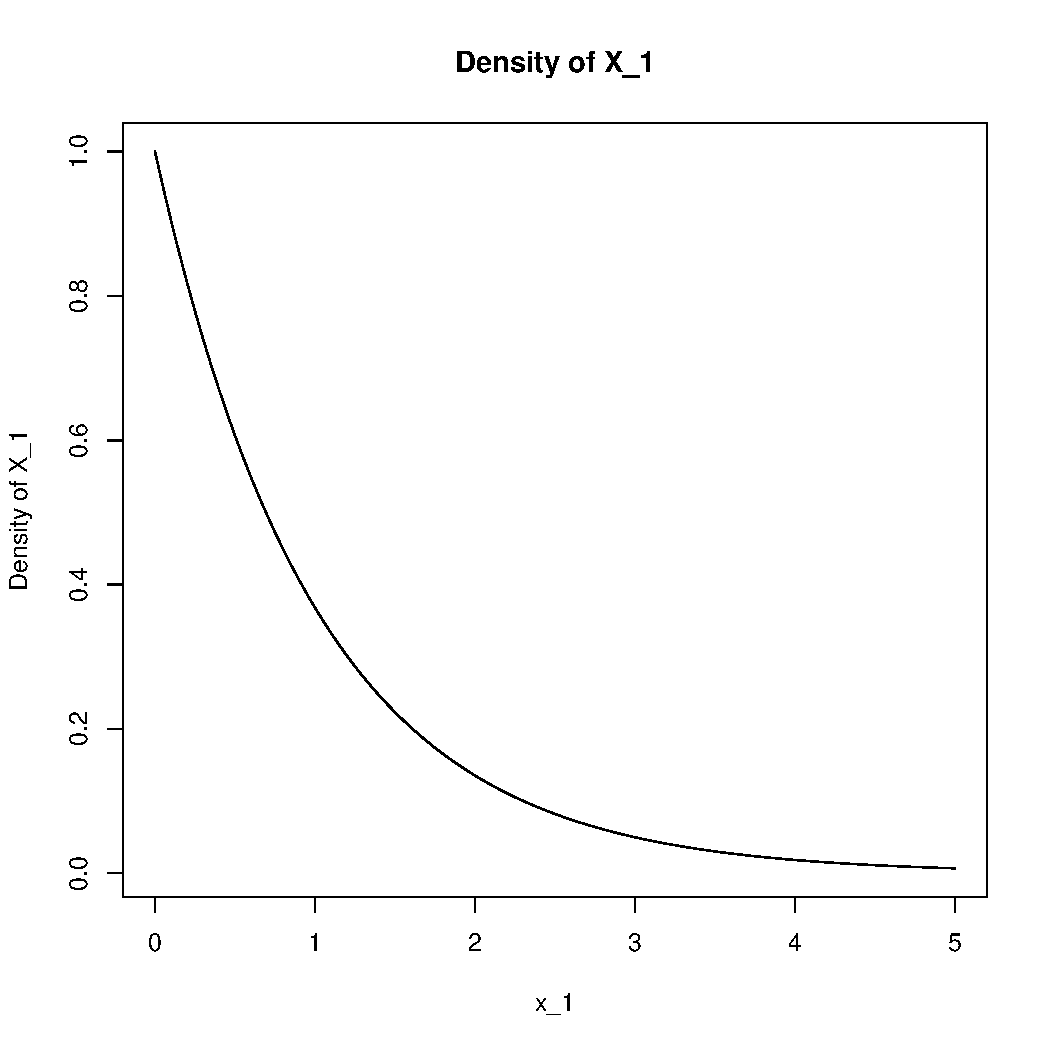
\includegraphics[width=.8\textwidth,height=.8\textheight]{figure/unnamed-chunk-2-1} 

\end{knitrout}
\end{frame}

\begin{frame}[fragile]
\frametitle{Example: cars}
\begin{knitrout}
\definecolor{shadecolor}{rgb}{0.969, 0.969, 0.969}\color{fgcolor}
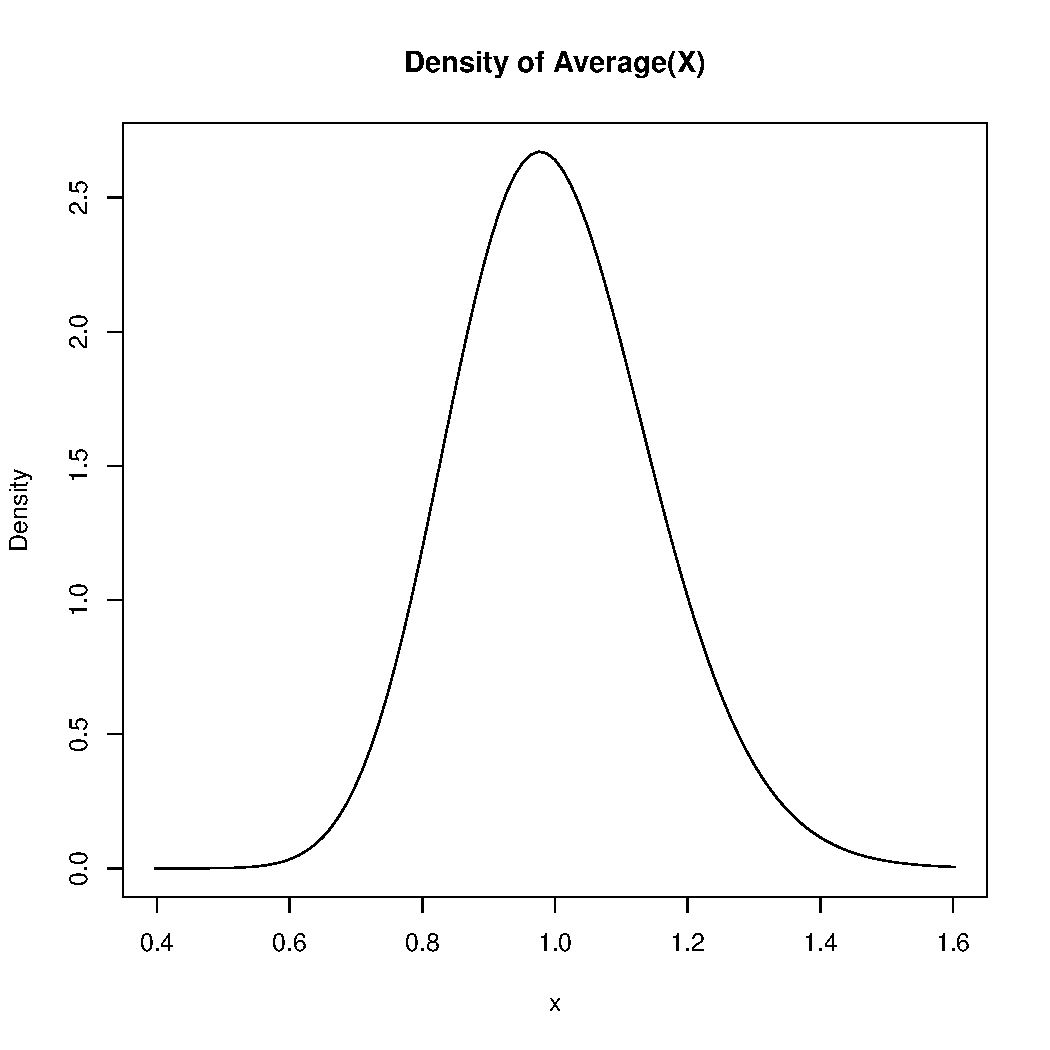
\includegraphics[width=.8\textwidth,height=.8\textheight]{figure/unnamed-chunk-3-1} 

\end{knitrout}
\end{frame}

\begin{frame}[fragile]
\frametitle{Example: cars}
\begin{knitrout}
\definecolor{shadecolor}{rgb}{0.969, 0.969, 0.969}\color{fgcolor}
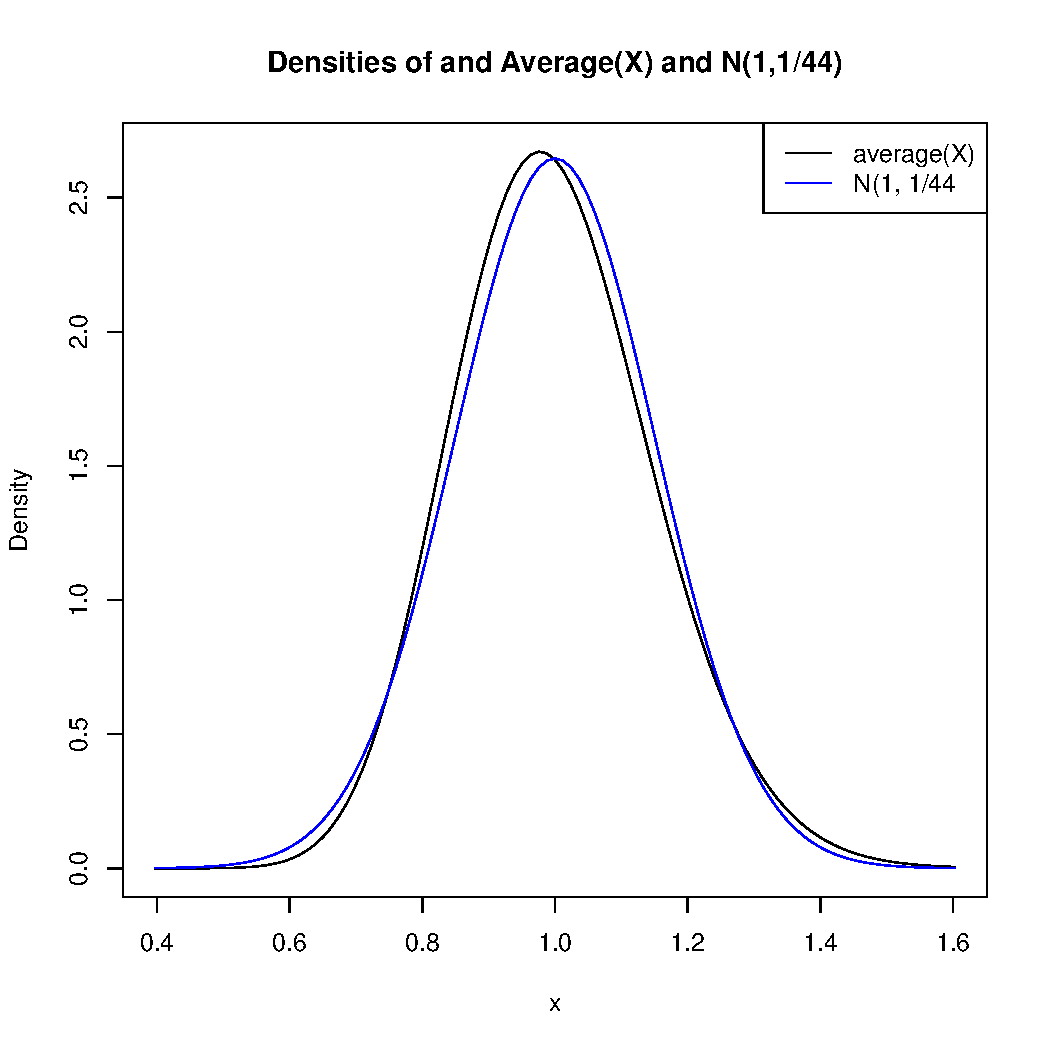
\includegraphics[width=.8\textwidth,height=.8\textheight]{figure/unnamed-chunk-4-1} 

\end{knitrout}
\end{frame}










\end{document}
